\documentclass[aspectratio=43]{beamer}
\usetheme{Berlin}

\usepackage[czech]{babel}
\usecolortheme{dolphin}
\usepackage{graphicx}
\usepackage{dirtree}
\usepackage{listings}
\usepackage[T1]{fontenc}
\usepackage{lmodern}
\usepackage[utf8]{inputenc}
\usepackage{caption}
\usepackage{bbding}
\usepackage{xurl}
\usepackage{scrextend}
\usepackage{minted}
\usepackage{appendixnumberbeamer}

\captionsetup{labelformat=empty}

\beamertemplatenavigationsymbolsempty
\defbeamertemplate*{title page}{customized}[1][]
{
	\usebeamerfont{title}\inserttitle\par
	\usebeamerfont{subtitle}\usebeamercolor[fg]{subtitle}\insertsubtitle\par
	\bigskip
	\usebeamerfont{author}\insertauthor\par
	\usebeamerfont{institute}\insertinstitute\par
	\usebeamerfont{date}\insertdate\par
	\usebeamercolor[fg]{titlegraphic}\inserttitlegraphic
}

\hypersetup{unicode}
\hypersetup{breaklinks=true}


\title{Bezpilotní letadlo}
\subtitle{Dron postavený na platformě Raspberry Pi}
\author{Havránek Kryštof 4.E}
\date{Březnen 2022}
\institute{Gymnázium, Praha 6, Arabská 14}
\setbeamertemplate{sidebar right}{}
\setbeamertemplate{footline}{%
\hfill\textbf{Stránka \insertframenumber{}. z \inserttotalframenumber} \hspace{0.01cm} \vspace{0.1cm}}
\setbeamerfont{footnote}{size=\tiny}

\begin{document}

\begin{frame}[plain]
	\maketitle
\end{frame}

\clearpage
\setcounter{framenumber}{0}

\begin{frame}[fragile]
	\frametitle{Úvod}
	\section{Úvod}

	\begin{itemize}
		\item Bezpilotní letadlo a jeho dobrovolný systém -- dálkové řízené, přenos videa a telemetrie
		\item Řízení přes Xbox ovladač
		\item Proč jsem si téma vybral?
		\item Kód dostupný na GitHubu pod licencí MIT (včetně knihoven)
		\item Linux + Raspbian, port ovládacího softwaru je možný
	\end{itemize}
\end{frame}

\begin{frame}[fragile]
	\frametitle{Protokol}
	\begin{itemize}
		\item Komunikace prostřednictvím protokolu postaveném na rodině TCP
		\item Video předáváno přes UDP (gstreamer)
		\item Protokol navržený pro potřeby práce -- tři základní funkce -- telemetrie, ovládání a nastavení
		\item Předávání struktur
		\item Raspberry Pi -- server, Pilot -- klient
		\item Podpora více ovládacích stanic
	\end{itemize}
\end{frame}

\begin{frame}[fragile]
	\frametitle{Design letadla}
	\section{Design letadla}
	\begin{itemize}
		\item Založeno na kostře Mini Talon od společnosti X-UAV
			\begin{itemize}
				\item Rozpětí křídel: 130cm
				\item Délka: 85cm
				\item Vzletová váha: 1.5 kg
			\end{itemize}
		\item Délka letu nad 1 hodinu
		\item Jádro -- Raspberry Pi Zero 2
		\item Doprovázen řadou periférií
	\end{itemize}
\end{frame}

\begin{frame}[fragile]
	\frametitle{Design letadla}
	\begin{figure}[h]
		\centering
		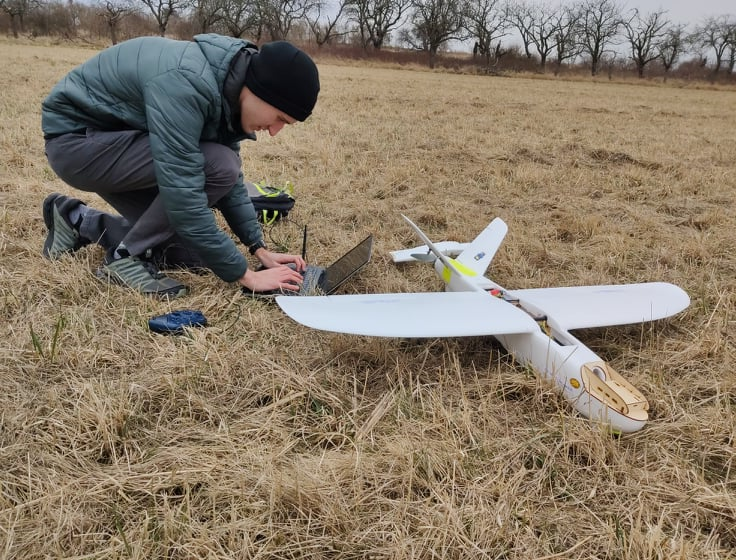
\includegraphics[height=7cm]{./../img/photo1.jpg}
	\end{figure}
\end{frame}

\begin{frame}[fragile]
	\frametitle{Design letadla}
	\begin{figure}[h]
		\centering
		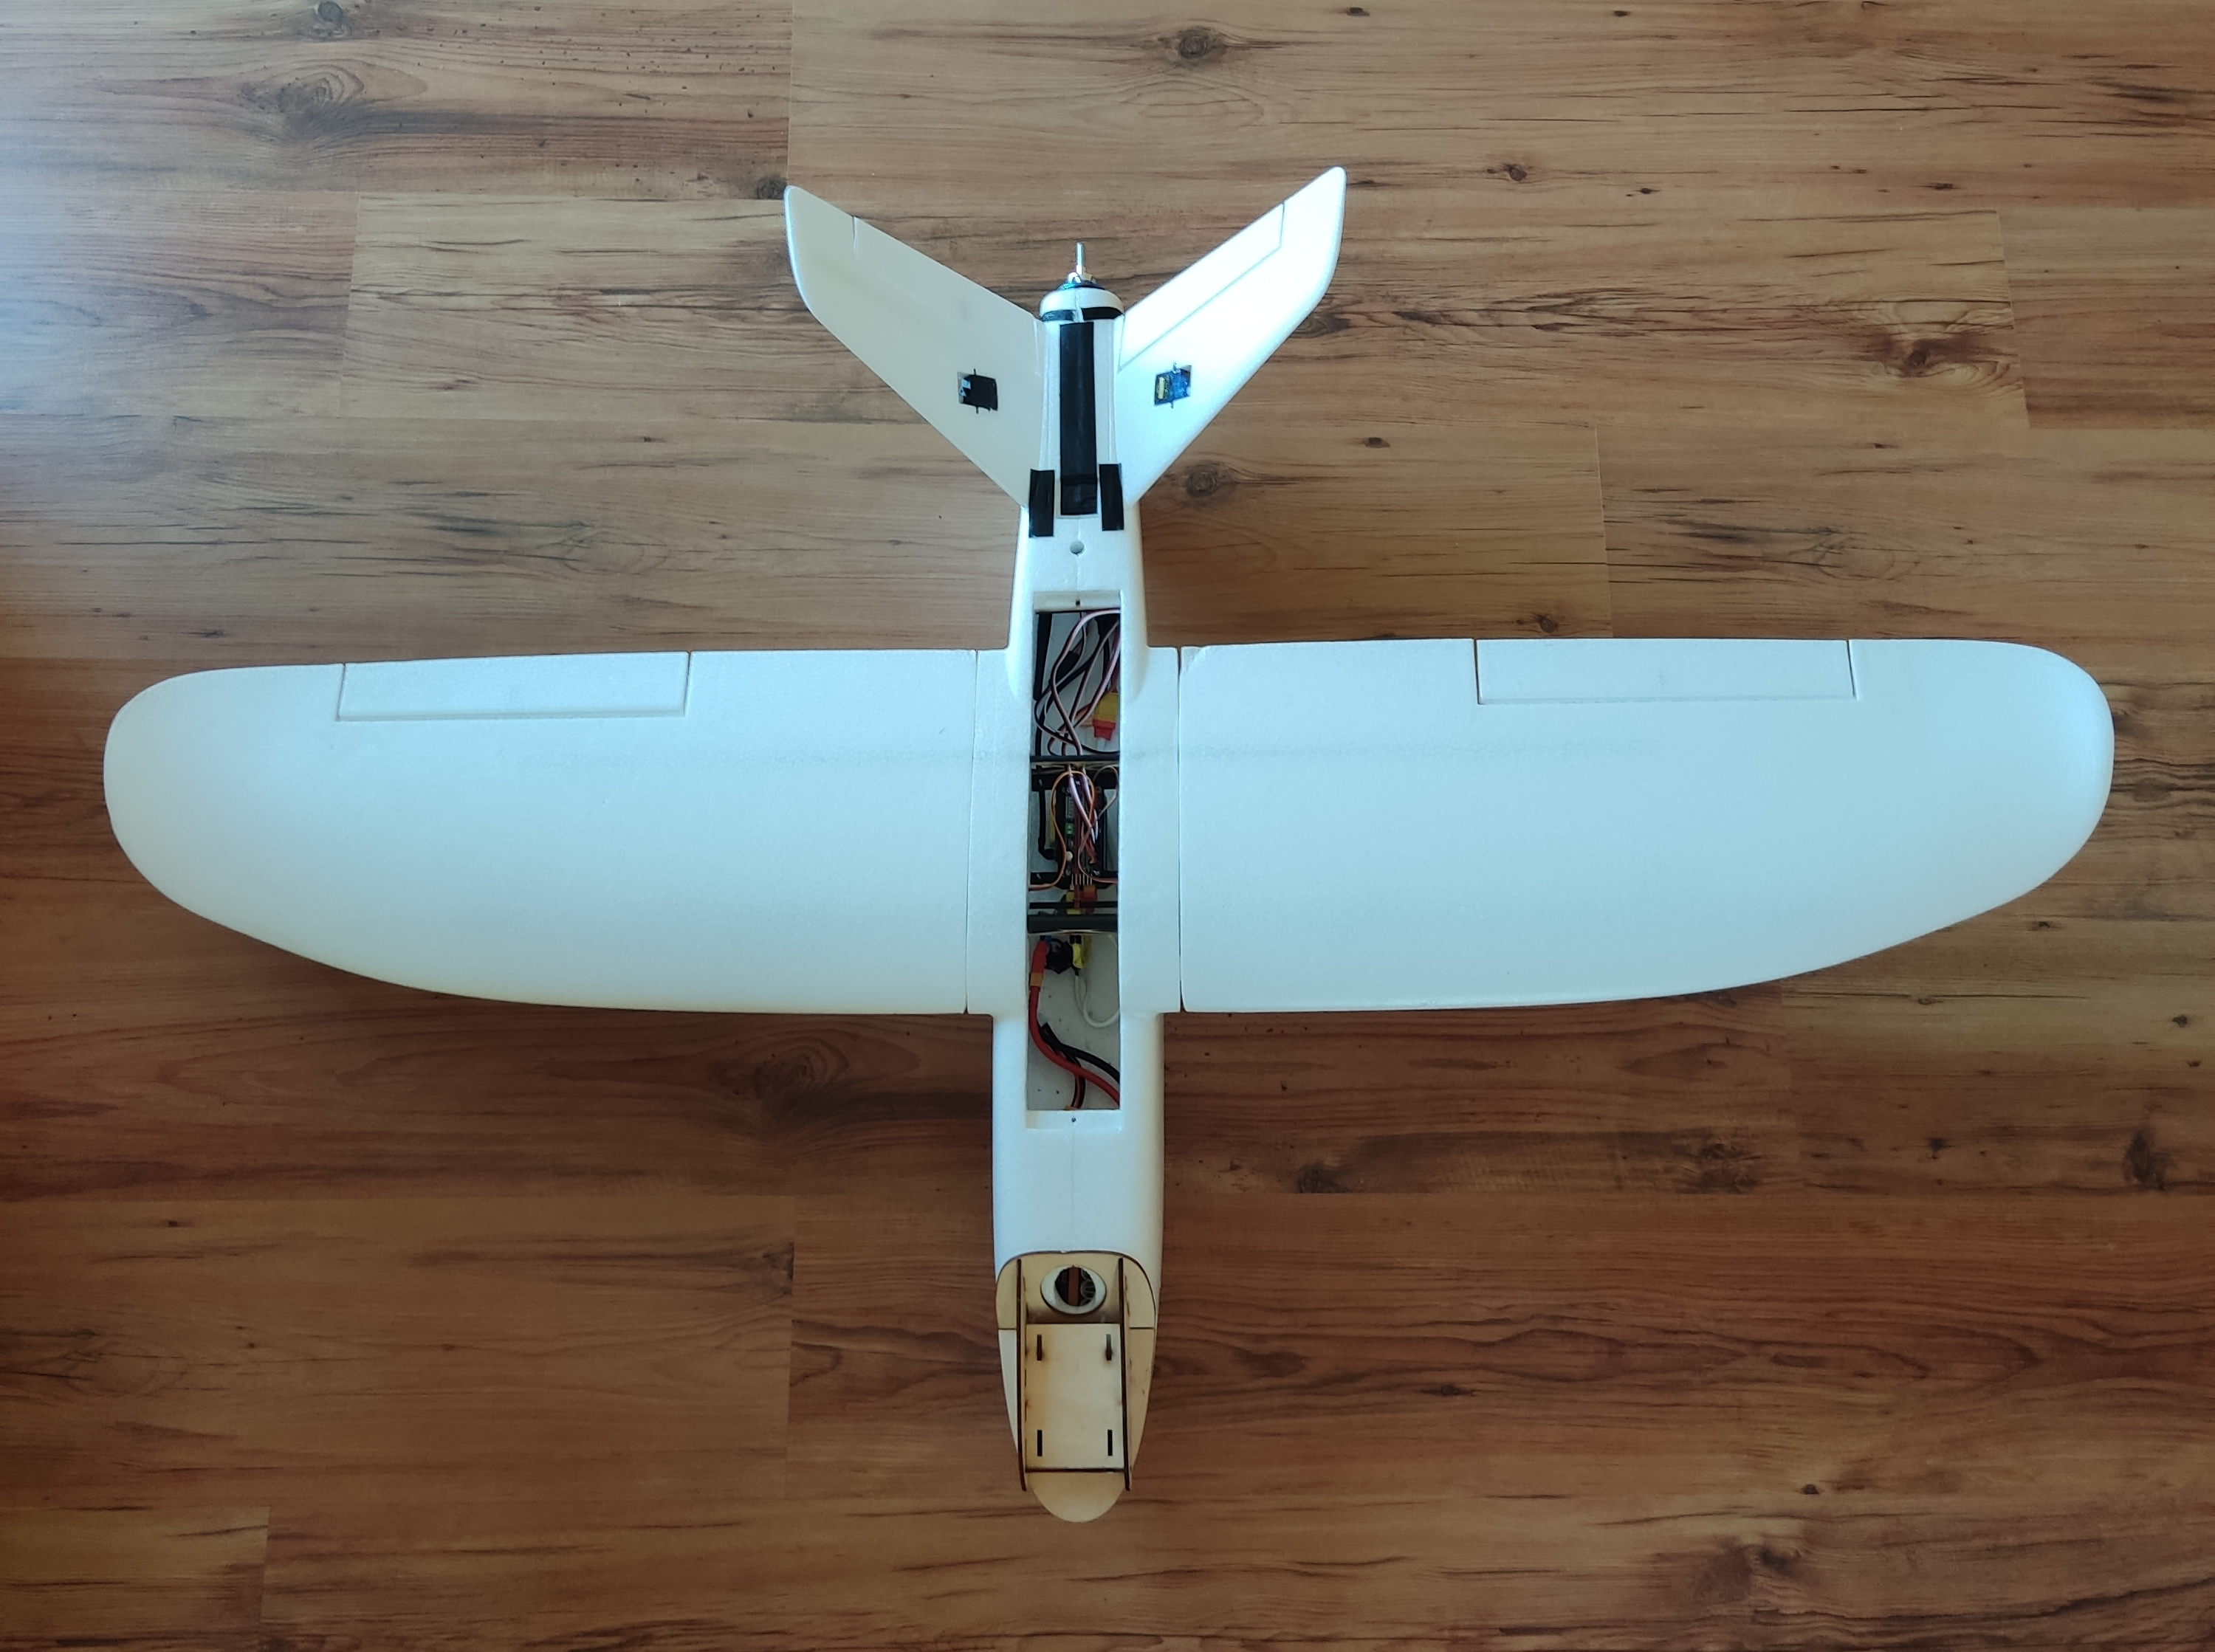
\includegraphics[height=7cm]{./../img/whole_plane.jpg}
	\end{figure}
\end{frame}


\begin{frame}[fragile]
	\frametitle{Periférie}
	\begin{itemize}
		\item Wit-Motion WT901B
			\begin{itemize}
				\item Devíti osý polohový senzor
				\item Údaje o orientaci v prostoru, teplotě, zrychlení
				\item Slouží k fungování autopilota
			\end{itemize}
		\item INA226
			\begin{itemize}
				\item Voltmetr/ampérmetr
				\item Měří odběr celého letadla a napětí na baterii
			\end{itemize}
	\end{itemize}
\end{frame}

\begin{frame}[fragile]
	\frametitle{Periférie}
	\begin{itemize}
		\item ublox NEO 7M
			\begin{itemize}
				\item GPS modul
				\item Údaje o poloze a nadmořské výšce
			\end{itemize}
		\item PCA9865
			\begin{itemize}
				\item Modul na ovládání servo motorů
				\item Připojen na ESC (Beatles 40A) -- ovládá rychlost hlavního motoru
			\end{itemize}
	\end{itemize}
\end{frame}

\begin{frame}[fragile]
	\frametitle{Zapojení}
	\begin{figure}[h]
		\centering
		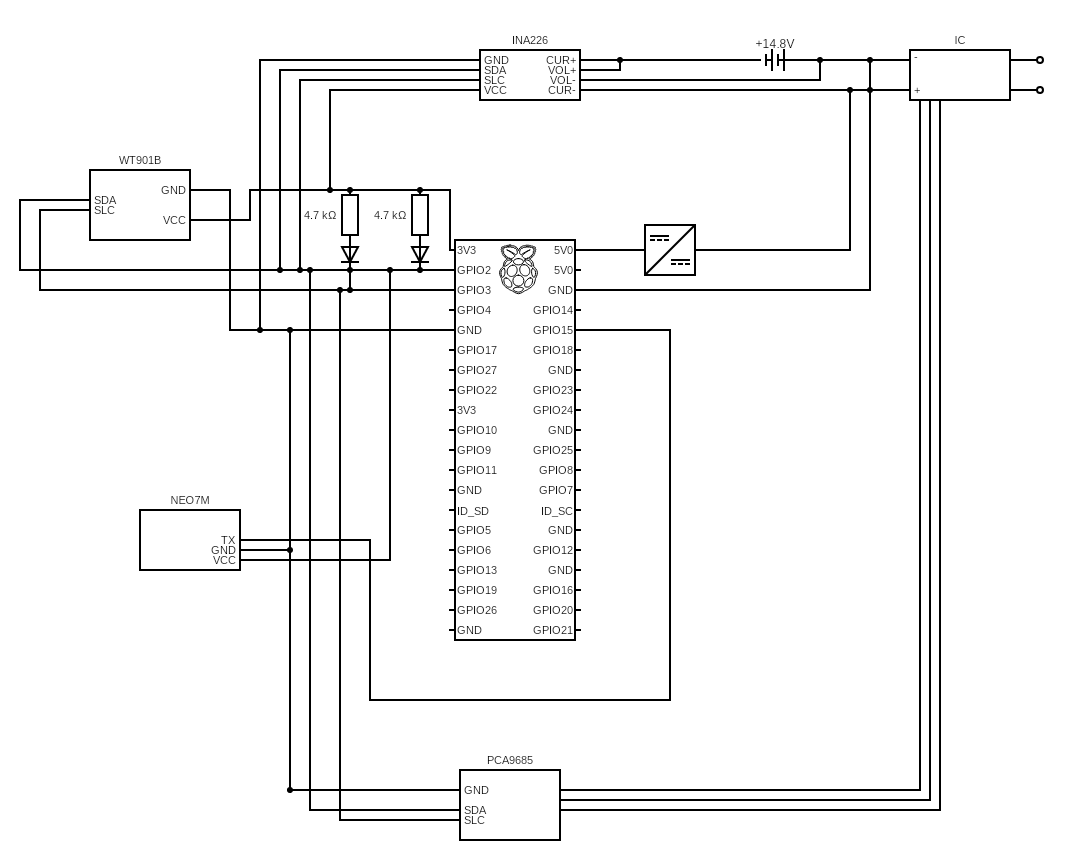
\includegraphics[height=7cm]{./../img/schema.png}
	\end{figure}
\end{frame}

\begin{frame}[fragile]
	\frametitle{Zapojení}
	\begin{figure}[h]
		\centering
		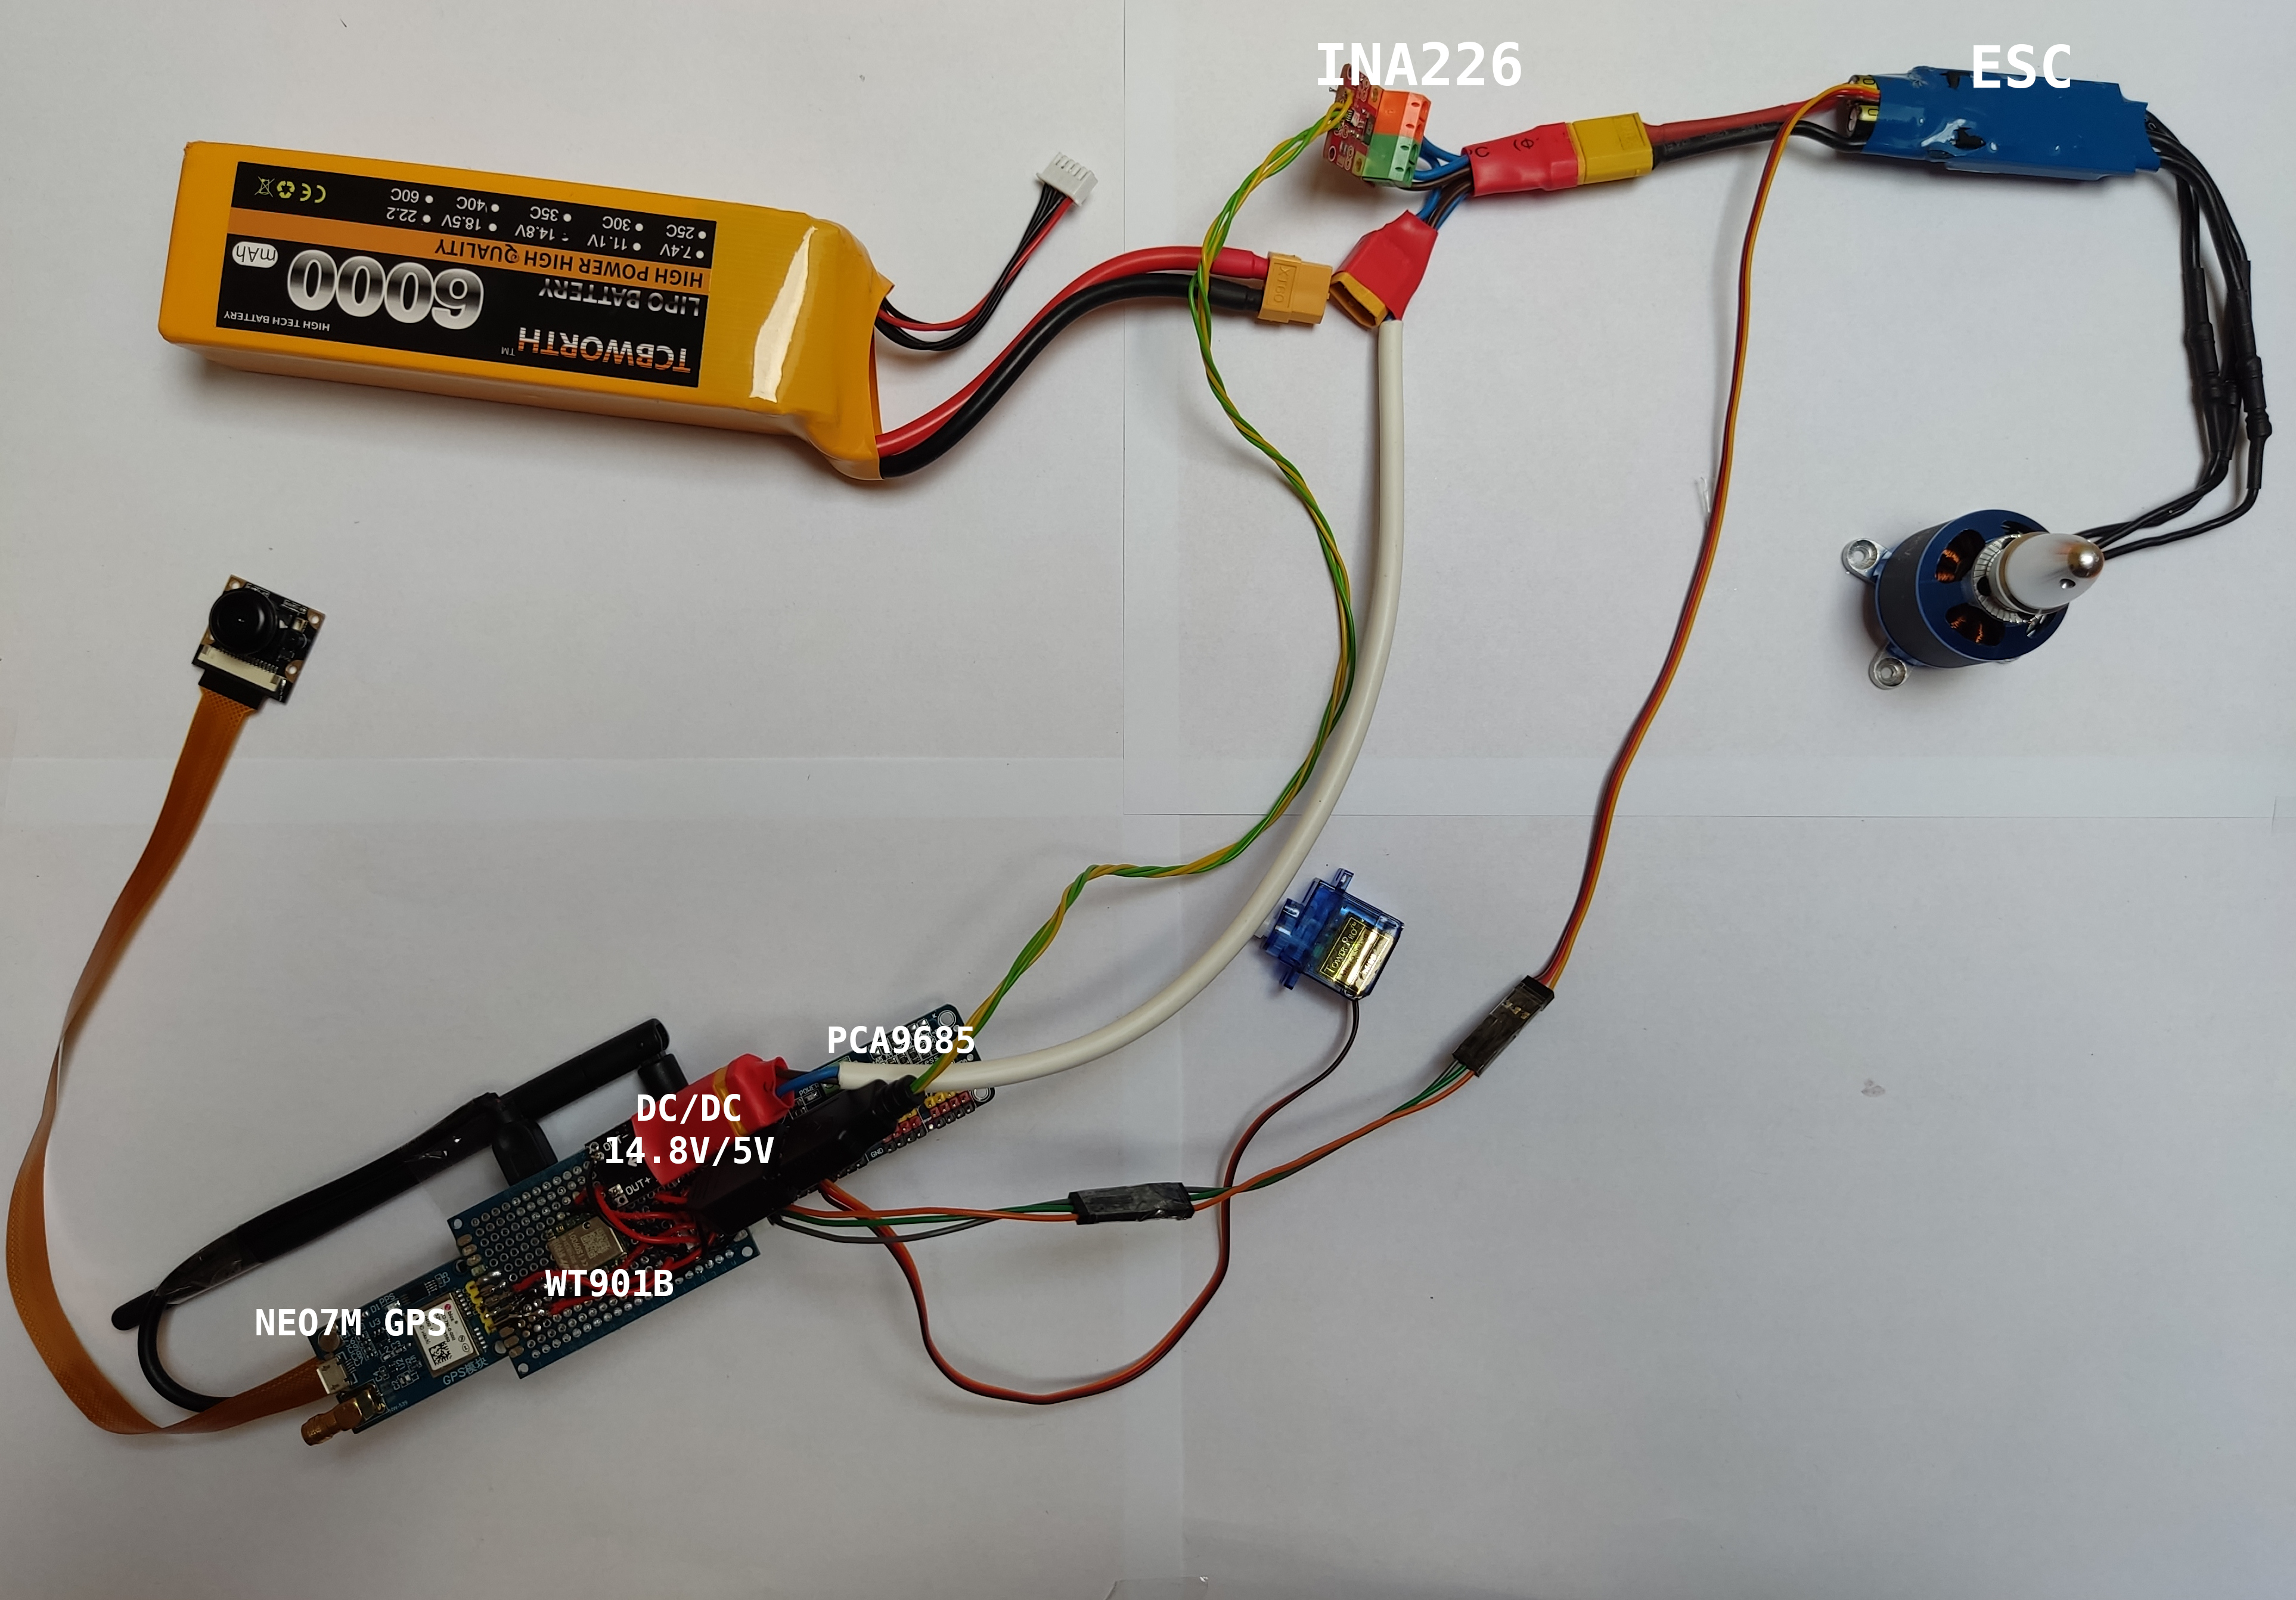
\includegraphics[height=7cm]{./../img/circuit.jpg}
	\end{figure}
\end{frame}

\begin{frame}[fragile]
	\frametitle{Program letadla}
	\begin{itemize}
		\item Se senzory se komunikuje prostřednictvím knihoven
			\begin{itemize}
				\item 3 forknuté a přepsané knihovny
				\item V programu se přistupuje přes singletony
			\end{itemize}
		\item Stream z kamery je aktuálně spuštěn programem v podprocesu
		\item Za standardního provozu se letadlo řídí pokyny pilota
		\item Čekání na zprávu $\Rightarrow$ vyhodnocení $\Rightarrow$ thread pool zpracuje
		\item Letadlo je schopno držet svojí letovou hladinu -- dva PID kontroléry
	\end{itemize}
\end{frame}

\begin{frame}[fragile]
	\frametitle{Ovládací software}
	\section{Ovládací software}
	\begin{itemize}
		\item Vyvíjen pro operační systém Linux
		\item Postavený na grafickém toolkitu Gtk3
		\item Zpracování dat z ovladače, zobrazení videa a telemetrie
		\item Ovladač
			\begin{itemize}
				\item Použit návrhový vzor observeru -- interface s ovladačem generuje události
				\item Nemusí tak existovat centrální organizační bod
				\item Odeslání příkazů letadlu, ovládání uživatelského prostředí
			\end{itemize}
	\end{itemize}
\end{frame}

\begin{frame}[fragile]
	\frametitle{Ovládací software}
	\begin{figure}[h]
		\centering
		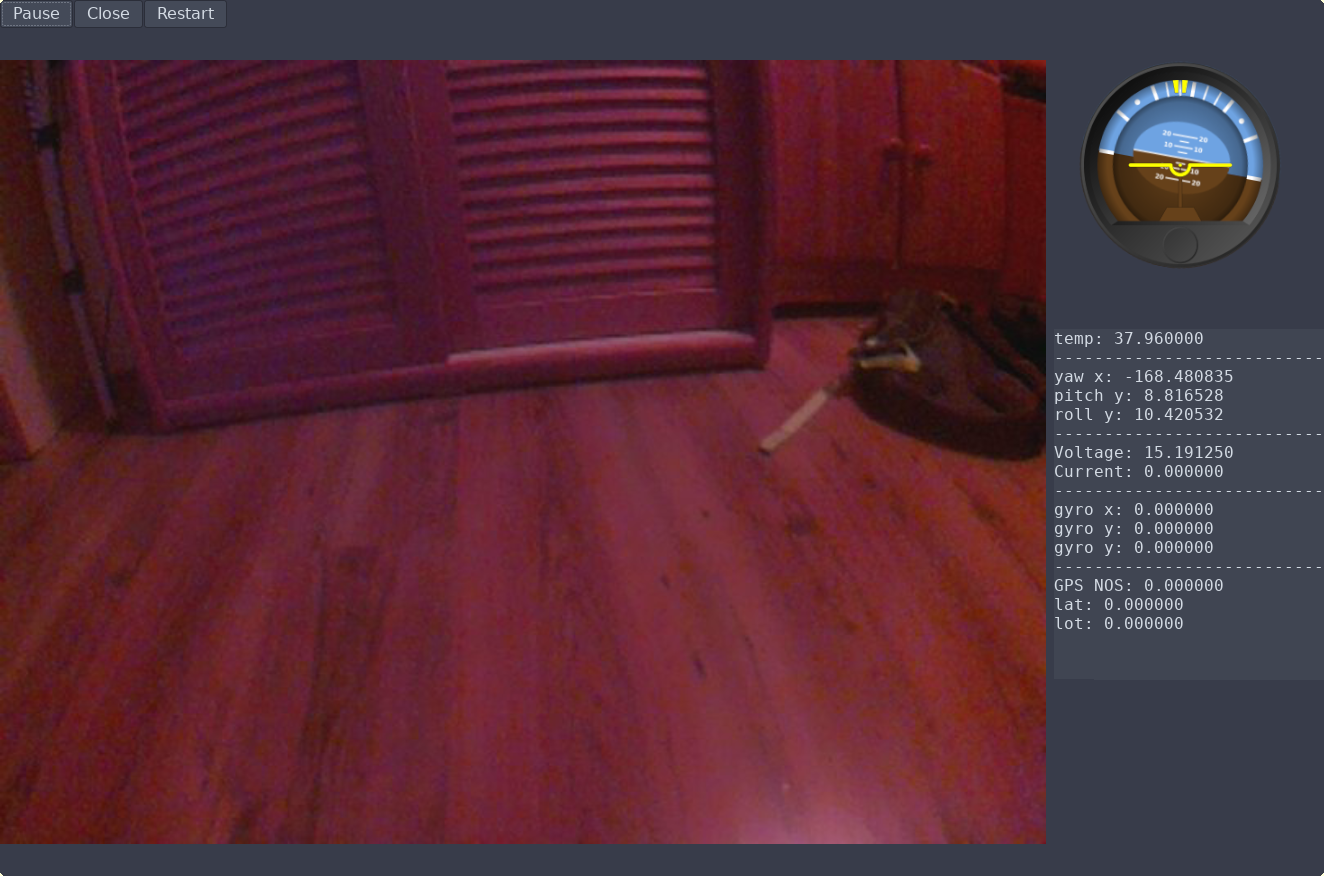
\includegraphics[height=7cm]{./../img/interface.png}
	\end{figure}
\end{frame}


\begin{frame}[fragile]
	\frametitle{Závěr}
	\section{Závěr}
	\begin{itemize}
		\item Cíl práce byl splněn
		\item Práce však nebyla realizována v původně zamýšleném rozsahu
		\item Řada problémů, kritický nedostatek znalostí
	\end{itemize}
\end{frame}

\begin{frame}[fragile]
	\frametitle{Budoucnost Projektu}
	\begin{itemize}
		\item Upozornění na letovou zónu
		\item Spojení s ATAK
		\item Autopilot
		\item Přechod od Wi-Fi, rezervní spojení?
		\item Doprovodný hardware -- tracking anténa, katapult
	\end{itemize}
\end{frame}

\appendix
\begin{frame}[plain]
	\centering
	\Huge Dotazy?
\end{frame}


\end{document}
